% Ubah judul dan label berikut sesuai dengan yang diinginkan.
\section{System Design}
\label{sec:systemdesign}

Our main program uses websites to interact with users because of its flexibility on any platform, the website view can be seen in Figure \ref{fig:websiteview}. So there is a Javascript client and a Python Server that communicate via \emph{socketio}.
The main program is divided into two modes, RECORD mode and PLAY mode. In RECORD mode, a human as a trainer gives a series of movements and will be followed by a humanoid robot, as well as robot save these movements to use in PLAY mode later.
Meanwhile, in the PLAY mode, the robot acts as a trainer and performs a series of movements according to the movements previously stored in RECORD mode. Human will follow the robot's movement while the robot is also saving both human and robot images.
So there will be two cameras, one camera to record human movement (located on the robot's head) and the other to record robot movement (located from the human side facing the robot), the distance between them approximately 1 - 1.5 meters, as shown in Figure \ref{fig:posecomparisonside}.
\begin{figure}[ht]
  \centering
  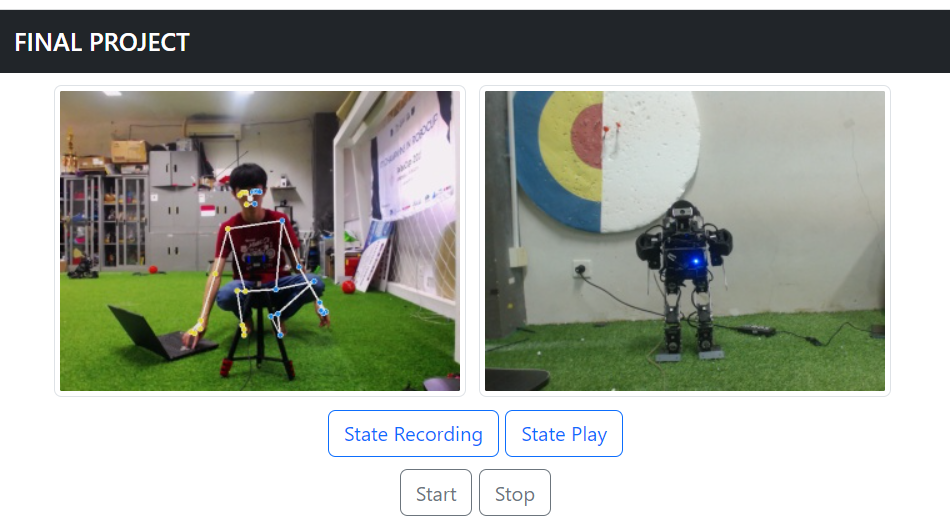
\includegraphics[width=0.48\textwidth]{gambar/web.png}
  \caption{Website View.}
  \label{fig:websiteview}
\end{figure}

\begin{figure}[ht]
  \centering
  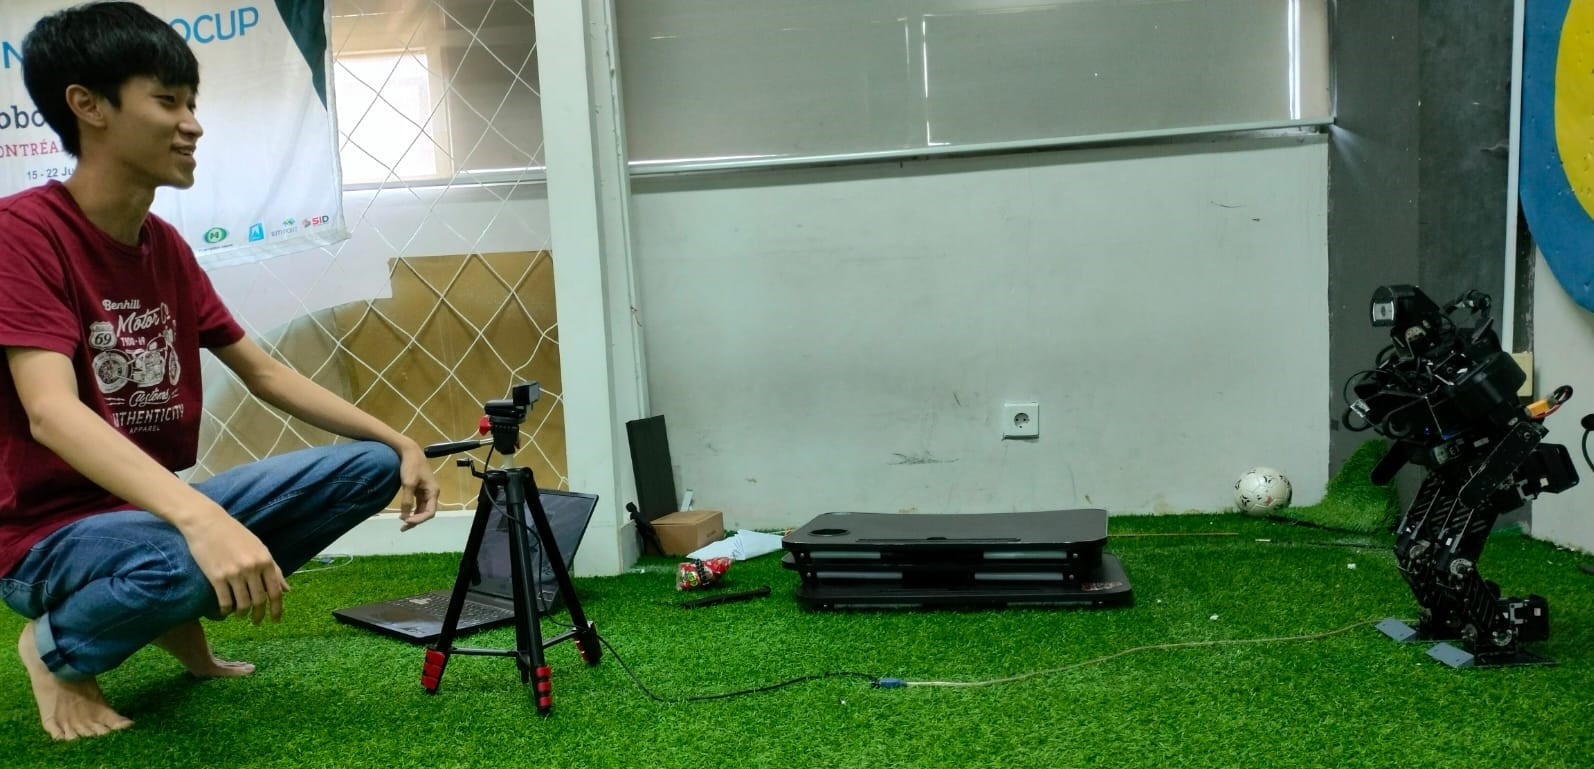
\includegraphics[width=0.47\textwidth]{gambar/pose-comparison.jpeg}
  \caption{Pose Comparison from Side.}
  \label{fig:posecomparisonside}
\end{figure}

On the client side, we use ReactJS framework. There are four buttons: RECORD, PLAY, START, and STOP button. The RECORD and PLAY button indicates the modes in the main program, while the START and STOP button tell us when the mode is started or stopped.
Besides that, there are also two images that show human and robot image that is sent from the server side. Client and server communicate through a predefined port.
We use the \emph{useEffect} function to indicate if there is a change in a particular variable and do something like converting the image from buffer to a string in order to display it on the HTML image tag later on and send some data to the server through clicking one of the buttons.

Meanwhile, our server uses ROS2 with Python language. To run the server and ROS2 program simultaneously, we need a separate thread, so the server program does not block the ROS2.
On this server side, all of the computations happen, starting from RECORD mode when Mediapipe detects human pose, visualizes the detection result, and send it as a buffer to the client.
Then, calculate each of the human's joint values, convert them to desired servo values in the real robot, communicate with other ROS2 packages to move the actual robot servo, and also save a series of human movements in a JSON file.
Whereas in PLAY mode, the server side sends two images so that we can know and adjust the position of humans and robots in the camera. Due to the large network delay when sending two 320x240 pixel images, when the START button is pressed,
the server does not send the image, the robot plays a series of moves stored in the previous JSON file by communicating via another ROS2 packages, while saving both images. After that, when the STOP button is pressed, the server starts to compare the suitability of poses between them.
